% ============================================================
% Parallel theory stream (articles/theory/) -- research note of
% record, typeset in the IDEG paper's own class (quantumarticle,
% two columns). Build: pdflatex -> bibtex -> pdflatex x2.
% Figures: figures/make_figures.py (numbers from checks/*.py).
% ============================================================
\RequirePackage[2023-06-01]{latexrelease}
\documentclass[a4paper,11pt,noarxiv]{quantumarticle}
\usepackage{amsmath,amssymb,amsthm}
\usepackage{graphicx}
\usepackage{booktabs}
\usepackage{array}
\usepackage{enumitem}
\usepackage{xcolor}
\definecolor{linkink}{HTML}{1c3f77}
\usepackage{hyperref}
\usepackage{microtype}
\emergencystretch=1.5em
\hypersetup{colorlinks=true,linkcolor=linkink,citecolor=linkink,
urlcolor=linkink}
\graphicspath{{figures/}}

\newcommand{\R}{\mathbb{R}}
\newcommand{\Rm}{R^{\mathrm m}}
\newcommand{\Risk}{\operatorname{Risk}}
\newcommand{\norm}[1]{\lVert #1\rVert}
\newcommand{\abs}[1]{\lvert #1\rvert}
\newcommand{\dd}{\,\mathrm{d}}
\newcommand{\grad}{\nabla}
\newcommand{\fbar}{\bar f}
\DeclareMathOperator{\capa}{cap}
\newcommand{\status}[1]{\textsc{\small [#1]}}

\theoremstyle{plain}
\newtheorem{proposition}{Proposition}
\newtheorem{lemma}[proposition]{Lemma}
\newtheorem{corollary}[proposition]{Corollary}
\newtheorem{theorem}[proposition]{Theorem}
\theoremstyle{definition}
\newtheorem{example}[proposition]{Example}
\newtheorem{restatement}[proposition]{Theorem}
\theoremstyle{remark}
\newtheorem{remark}[proposition]{Remark}

\title{Shrinkage priors, admissibility, and weighted Riemannian
geometry: a dictionary with status tags}
\author{Oleg Roshka}
\affiliation{Independent Researcher \textnormal{--}
\href{https://orcid.org/0009-0009-3075-9417}{ORCID
0009-0009-3075-9417}}
\date{23 October 2026}

\begin{document}
\maketitle

\begin{abstract}
Two literatures touch without citing each other: Stein-type shrinkage
and admissibility (Stein, Brown, Komaki) and the potential theory of
weighted Riemannian manifolds (Grigor'yan; Perelman's weighted scalar
curvature). This note records the contact points, each with a status
tag. (i)~Komaki's $O(N^{-2})$ risk reduction of a prior
$e^{-\Phi}\pi_J$ over the Jeffreys prior equals $(\Rm_\Phi-R)/(2N^2)$,
the $\Phi$-dependent part of Perelman's weighted scalar curvature; the
$R$ term has no statistical counterpart. (ii)~Brown's 1971
admissibility theory is the potential theory of the weighted Euclidean
space $(\R^m,\delta,f^*\dd x)$: his Theorem~5.1.1 reads ``admissible
if and only if parabolic'', and his 1971 sphere-average test is the
sphere-area parabolicity test that the geometric literature attributes
to Lyons--Sullivan (1984) and Grigor'yan (1985). (iii)~Two elementary
lemmas locate the cases that Brown's radial tests leave open: a bounded
spherical $A_2$ ratio makes his two tests exhaustive, and for product
weights the doubling and Poincar\'e hypotheses of heat-kernel theory
force that bound, so a volume-growth criterion decides nothing new
there. An explicit undecided example is settled (inadmissible) by
product heat kernels, an instance of Johnstone--Lalley (1984). No
dynamical and no gravitational claim is made.
\end{abstract}

\section{Scope and status}\label{sec:scope}

This is a research note of record, written to close a question rather
than to open a field. It replaces an LLM-drafted blueprint that read
the same material as ``emergent spacetime''; twenty-two machine checks
found six of that blueprint's displayed equations wrong, and the
present text keeps only what survived against the primary sources.
Every claim carries one of four tags. \status{theorem}: stated and
proved in the cited source, which we read. \status{identity}: an
elementary identity, re-derived symbolically in the check scripts.
\status{negative}: a conjecture of the blueprint refuted from a source.
\status{observation}: sourced on both sides, novelty not established.
For novelty the only permitted wording is ``not found in the literature
we searched''; a citation-index sweep has not been run.

\begin{figure*}[t]
\centering
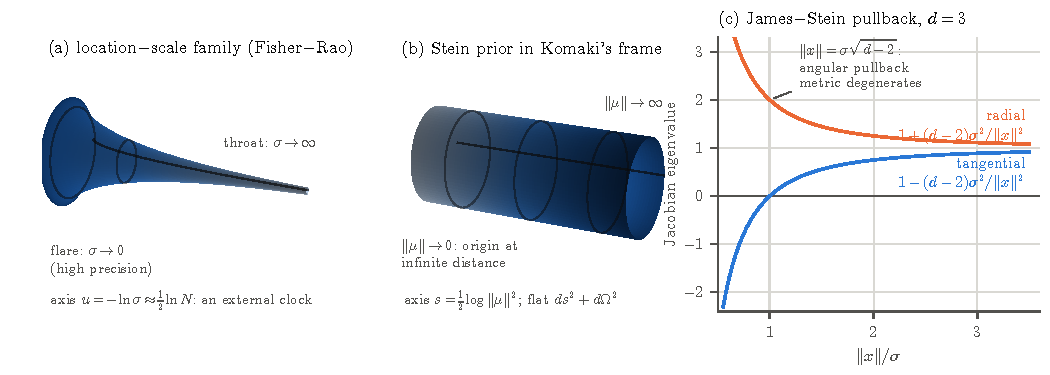
\includegraphics[width=\textwidth]{fig1_geometries.pdf}
\caption{Three of the four geometries of \S\ref{sec:geoms}. (a) The
Fisher--Rao metric of a location--scale family, hyperbolic, drawn as
the pseudosphere (curvature $-1$ after rescaling): throat
$\sigma\to\infty$, flare $\sigma\to0$, axial coordinate
$-\ln\sigma\approx\tfrac12\ln N$, an external clock; the meridian is a
geodesic. (b) Komaki's conformal frame of the Stein prior: the flat
cylinder $S^{d-1}\times\R$ (sphere drawn as a circle) with the origin
pushed to infinite distance; constant cross-section, no horizon.
(c) Jacobian eigenvalues of the James--Stein map for $d=3$: the
tangential eigenvalue vanishes at $\norm x=\sigma\sqrt{d-2}$, where the
estimator's pullback metric degenerates in the angular directions.
Shading encodes the axial coordinate.}
\label{fig:geom}
\end{figure*}

Sources read in full or in the cited parts: Brown~\cite{brown1971},
Komaki~\cite{komaki2006,komaki2015}, Perelman~\cite{perelman2002}
(\S1), Grigor'yan~\cite{grigoryan1999} (\S\S3, 5, 7, 11),
Johnstone~\cite{johnstone2019}, George--Liang--Xu~\cite{glx2006},
Maruyama--Strawderman~\cite{maruyama2021},
Takanashi--McAlinn~\cite{takanashi2023}. Works marked ``not accessed''
in the bibliography are quoted as recalled; nothing below depends on
them except the heat-kernel remark of \S\ref{sec:reach}, which is
explicitly conditional, and the Poincar\'e column of
Table~\ref{tab:weights}, which uses Muckenhoupt's weighted Hardy
inequality.

\section{Setting}\label{sec:setting}

\paragraph{Model side.}
A regular model $\{p(x\mid\theta):\theta\in\Theta\subset\R^d\}$ carries
the Fisher metric $g_{ij}=E[\partial_i\ell\,\partial_j\ell]$, the
Jeffreys prior $\pi_J\propto\abs{g}^{1/2}$ and the Laplace--Beltrami
operator $\Delta_g$ \cite{amari2000}. A smooth prior is written
$f=e^{-\Phi}\pi_J$, and $u=\sqrt{f/\pi_J}=e^{-\Phi/2}$. The pair
$(g,\Phi)$ defines the smooth metric measure space
$(M,g,e^{-\Phi}\dd V)$ with weighted Laplacian
$\Delta_\Phi=\Delta_g-\grad\Phi\cdot\grad$, self-adjoint on
$L^2(e^{-\Phi}\dd V)$, Bakry--\'Emery tensor
$\mathrm{Ric}+\grad\grad\Phi$ \cite{bakryemery1985}, and Perelman's
weighted scalar curvature \cite{perelman2002}
\begin{equation}\label{eq:perelman}
\Rm_\Phi=R+2\Delta_g\Phi-\abs{\grad\Phi}_g^2,
\end{equation}
whose integral is his functional
$\mathcal F(g,\Phi)=\int\Rm_\Phi\,e^{-\Phi}\dd V
=\int(R+\abs{\grad\Phi}^2)e^{-\Phi}\dd V$.
A weighted manifold is \emph{parabolic} if its weighted Brownian motion
is recurrent, equivalently if it carries no Green function and no
nonconstant positive superharmonic function \cite[\S5]{grigoryan1999}.
$\Risk_N(f)$ is the Kullback--Leibler risk of the Bayesian predictive
density built from $N$ observations under the prior $f$.

\paragraph{Brown's side.}
$X\sim N_m(\theta,I)$, $F$ a $\sigma$-finite prior on $\R^m$,
$f^*=p*F$ its marginal (here $p$ is the normal density), and
$\delta_F=x+\grad\log f^*=x+\gamma_F$ the generalized Bayes estimator;
$\delta_F$ has bounded risk when $\gamma_F$ is bounded
\cite[\S3]{brown1971}. We write $W_F=(\R^m,\delta_{ij},f^*\dd x)$ for
the weighted Euclidean space. Brown's diffusion $\{Z_t\}$, with
generator $\Delta+\grad\log f^*\cdot\grad$ up to a constant factor, is
the weighted Brownian motion of $W_F$. For $r\ge1$ let $\fbar(r)$ and
$A(r)$ be the means of $f^*$ and of $1/f^*$ over the sphere
$\{\abs{x}=r\}$, and $Q(r)=\fbar(r)A(r)\ge1$ the \emph{spherical $A_2$
ratio}.

\section{Shrinkage priors and the weighted scalar curvature}
\label{sec:komaki}

\begin{proposition}[\status{identity} on \status{theorem} inputs]
\label{prop:k1}
For a regular model and $f=e^{-\Phi}\pi_J$, the risk reduction
$\varrho_N(f)=\Risk_N(\pi_J)-\Risk_N(f)$ satisfies
\begin{multline}\label{eq:k1}
\varrho_N(f)
=\frac{1}{2N^2}\bigl(2\Delta_g\Phi-\abs{\grad\Phi}_g^2\bigr)+o(N^{-2})\\
=\frac{\Rm_\Phi-R}{2N^2}+o(N^{-2})\\
=-\frac{2}{N^2}\,\frac{\Delta_g u}{u}+o(N^{-2}).
\end{multline}
The prior $f$ asymptotically dominates $\pi_J$ if and only if $u$ is a
nonconstant positive superharmonic function on $(M,g)$, that is, if and
only if $\Rm_\Phi\ge R$ with strict inequality somewhere.
\end{proposition}

\begin{proof}
The first equality is Komaki's expansion \cite[eqs.\ (3)--(5)]{komaki2006}:
in the difference of two priors the skewness terms and the
prior-independent terms cancel. The second is the definition
\eqref{eq:perelman} with $f\equiv\Phi$ \cite[Remark 1.3]{perelman2002};
the third is the identity $2\Delta\Phi-\abs{\grad\Phi}^2=-4\Delta u/u$
for $u=e^{-\Phi/2}$. The domination statement is Komaki's Theorem~2.
(The blueprint had the sign of the first line reversed; checks C8--C10.)
\end{proof}

\begin{proposition}[\status{negative}]\label{prop:k2}
The prior-independent $O(N^{-2})$ term of the Jeffreys predictive risk
is not proportional to the scalar curvature $R$ of $(M,g)$, and
$\mathcal F$ is not the integrated predictive risk. Whenever the
boundary term of one integration by parts vanishes, up to $o(N^{-2})$,
\begin{multline}\label{eq:k2}
\int\varrho_N(f)\,e^{-\Phi}\dd V
=\frac{1}{2N^2}\int\abs{\grad\Phi}_g^2\,e^{-\Phi}\dd V\\
=\frac{1}{2N^2}\Bigl[\mathcal F(g,\Phi)-\int R\,e^{-\Phi}\dd V\Bigr].
\end{multline}
\end{proposition}

\begin{proof}
Komaki \cite[Theorem A1, eq.\ (29)]{komaki2015} writes the full
$O(N^{-2})$ risk. Its prior-independent part is a fixed combination of
the exponential and mixture embedding curvatures, the skewness norm
$T_{ijk}T^{ijk}$, a fourth-moment contraction and one mixed moment. For
$d=1$ these are generically nonzero (Efron's statistical curvature of
a curved exponential family \cite{efron1975}), while every intrinsic
curvature of a one-dimensional Riemannian manifold vanishes. Equation
\eqref{eq:k2} follows from \eqref{eq:k1} and
$\int\Delta\Phi\,e^{-\Phi}\dd V=\int\abs{\grad\Phi}^2e^{-\Phi}\dd V$.
\end{proof}

So only the gradient part of $\mathcal F$ is statistical, and the
operator that governs shrinkage domination is $-4\Delta_g$ acting on
$u$: Perelman's operator $-4\Delta+R$ with the potential removed. His
eigenvalue $\lambda(g)$ has no reading here.

\begin{remark}[\status{theorem}, Komaki]\label{rem:k3}
Komaki's Theorems~1--2 \cite{komaki2006} say that a prior
asymptotically dominating $\pi_J$ exists if and only if $(M,g)$ carries
a Green function, i.e.\ is non-parabolic; his Theorem~3 obtains this
from negative sectional curvature for $d\ge3$ via Aomoto
\cite{aomoto1966}. For the flat normal location model the Green
function exists iff $d\ge3$ and the Green prior is Stein's harmonic
prior $\norm{\mu}^{-(d-2)}$ (Komaki's Example~1). Curvature enters
statistics here, through transience, and not through $R$ in the risk.
\end{remark}

\begin{proposition}[\status{theorem} + \status{identity}]\label{prop:k5}
For $d\ge3$ and a vague prior $h=e^{-\Phi}\pi_J$, Komaki
\cite[\S3, Theorems 4--6]{komaki2006} decides domination over $h$ by
superharmonicity on the conformal metric
$\tilde g=(h/\pi_J)^{2/(d-2)}g=e^{-2\Phi/(d-2)}g$. In that frame,
up to boundary terms,
\begin{equation}\label{eq:frame}
\mathcal F(g,\Phi)=\int\Bigl[\tilde R-\tfrac{1}{d-2}\,
\abs{\tilde\grad\Phi}^2_{\tilde g}\Bigr]\dd\tilde V,
\end{equation}
(check C2; the blueprint's coefficient $(d-1)/(d-2)$ was wrong). For
the Stein prior the frame is the flat cylinder $S^{d-1}\times\R$ under
$\mu\mapsto(\mu/\norm{\mu},\tfrac12\log\norm{\mu}^2)$, with the origin
at infinite distance (Komaki's Example~1; Fig.~\ref{fig:geom}b).
\end{proposition}

In words: changing the vague prior is a conformal change of the Fisher
metric. The ``dilaton'' form of \eqref{eq:frame} is a name for a
static Riemannian functional and carries no further content.

\section{Brown (1971) as potential theory on \texorpdfstring{$W_F$}{W\_F}}
\label{sec:brown}

\begin{restatement}[Brown \cite{brown1971}, restated; \status{theorem} on both sides]
\label{thm:brown}\leavevmode
\begin{enumerate}[label=\textup{(\alph*)},leftmargin=1.7em,itemsep=2pt,topsep=2pt]
\item (Thm.\ 4.3.1) $\{Z_t\}$ is transient iff the infimum of
$\int\abs{\grad j}^2f^*\dd x$ over compactly supported $j$ with $j=1$
on $\abs x\le1$ is positive, i.e.\ iff $\capa_{W_F}(B_1)>0$:
non-parabolicity of $W_F$ \cite[Thm.\ 5.1(6)]{grigoryan1999}.
\item (Thm.\ 5.1.1) If $\gamma_F$ is bounded, $\delta_F$ is admissible
iff $W_F$ is parabolic; transience implies inadmissibility with no
condition.
\item (Thm.\ 6.3.1) For spherically symmetric $F$, $\delta_F$ is
inadmissible iff $\int_1^\infty\dd r/(r^{m-1}f^*(r))<\infty$: the
model-manifold test $\int^\infty\dd r/S(r)$
\cite[Prop.\ 3.1]{grigoryan1999} for the weighted sphere area
$S(r)=\omega_{m-1}r^{m-1}f^*(r)$ (check C23).
\item (Thm.\ 6.4.3) For any $F$,
$\int_1^\infty\dd r/(r^{m-1}\fbar(r))=\infty$ implies that $W_F$ is
parabolic, hence $\delta_F$ admissible when $\gamma_F$ is bounded: the
sphere-area test \cite[Thm.\ 7.5]{grigoryan1999}.
\item (Thm.\ 6.4.4) If a set $\Omega$ of directions of positive
surface measure has
$\sup_{\varphi\in\Omega}\int_1^\infty\dd r/(r^{m-1}f^*(r\varphi))<\infty$,
then $\delta_F$ is inadmissible.
\item (Thm.\ 6.4.2) Under $\abs{\gamma_F(x)}\le k/\abs{x}$ the test in
(d) is an equivalence.
\end{enumerate}
\end{restatement}

Brown's proofs are those of the geometric statements: (a) is his
energy integral and variational problem, (d) is the radial test
function built from $1/(r^{m-1}\fbar)$, and (e) integrates the
one-dimensional capacity bound along rays. Table~\ref{tab:dict}
collects the dictionary.

\begin{table*}[t]
\caption{Dictionary, with status. Theorem numbers refer to
Brown~\cite{brown1971}, Komaki~\cite{komaki2006} and
Grigor'yan~\cite{grigoryan1999}.}
\label{tab:dict}
\small
\begin{tabular}{@{}>{\raggedright\arraybackslash}p{0.33\textwidth}>{\raggedright\arraybackslash}p{0.37\textwidth}>{\raggedright\arraybackslash}p{0.24\textwidth}@{}}
\toprule
statistics & weighted Riemannian geometry & status \\
\midrule
model manifold with Fisher metric $(M,g)$ & Riemannian manifold & definition \cite{amari2000} \\
prior $f=e^{-\Phi}\pi_J$ & smooth metric measure space $(M,g,e^{-\Phi}\dd V)$ & definition \\
$O(N^{-2})$ risk reduction over Jeffreys & $(\Rm_\Phi-R)/(2N^2)=-2\Delta u/(N^2u)$ & identity (Prop.~\ref{prop:k1}) \\
asymptotic domination over Jeffreys (Komaki Thm.\ 2) & $u$ nonconstant positive superharmonic & theorem \\
a shrinkage prior exists (Komaki Thm.\ 1) & $(M,g)$ non-parabolic & theorem \\
prior-independent $O(N^{-2})$ risk & embedding curvatures, skewness, fourth moment; \textbf{not} $R$ & negative (Prop.~\ref{prop:k2}) \\
change of vague prior $h$ (Komaki \S3) & conformal change $\tilde g=(h/\pi_J)^{2/(d-2)}g$ & theorem (Prop.~\ref{prop:k5}) \\
Stein prior in Komaki's frame & flat cylinder $S^{d-1}\times\R$, origin at infinity & theorem (Komaki Ex.\ 1) \\
$\delta_F$ admissible, bounded risk (Brown Thm.\ 5.1.1) & $W_F=(\R^m,\delta,f^*\dd x)$ parabolic & theorem \\
Brown's energy infimum (Thm.\ 4.3.1) & capacity of the unit ball in $W_F$ (Grig.\ Thm.\ 5.1) & theorem \\
Brown Thm.\ 6.3.1 (spherical $F$) & model-manifold test $\int\dd r/S(r)$ (Grig.\ Prop.\ 3.1) & theorem (C23) \\
Brown Thm.\ 6.4.3 (any $F$) & sphere-area parabolicity test (Grig.\ Thm.\ 7.5) & theorem; Remark~\ref{rem:k7} \\
--- & ball-volume test $\int\rho\dd\rho/V(\rho)=\infty$ (Grig.\ Thm.\ 7.3) & corollary of 6.4.3, weaker (C24) \\
MLE admissible iff $m\le2$ (Stein \cite{stein1956}) & Brownian motion recurrent iff $m\le2$ & theorem ($f^*\equiv1$) \\
Bakry--\'Emery flow $\partial_tg=-2(\mathrm{Ric}+\grad\grad\Phi)$ & gradient flow of $\mathcal F$ at fixed measure & theorem (Perelman), no statistical process (\S\ref{sec:geoms}) \\
\bottomrule
\end{tabular}
\end{table*}

\begin{corollary}[\status{identity}, check C24]
The ball-volume test $\int^\infty\rho\dd\rho/\mu(B_\rho)=\infty$
\cite[Thm.\ 7.3]{grigoryan1999} follows from Theorem~\ref{thm:brown}(d)
by the Cauchy--Schwarz inequality on dyadic shells, and is strictly
weaker.
\end{corollary}

\begin{remark}[\status{observation}: priority]\label{rem:k7}
Grigor'yan \cite[p.~178]{grigoryan1999} attributes the sphere-area test
for Riemannian manifolds to Lyons--Sullivan \cite{lyonssullivan1984}
and Grigor'yan \cite{grigoryan1985}. Brown's Theorem~6.4.3 (1971) is
the same test on $W_F$, and his Theorem~4.3.1 is the capacity
characterization of parabolicity. In the sources we read neither
literature cites the other. The analytic content of
Theorem~\ref{thm:brown}(a)--(b), admissibility as recurrence of the
Dirichlet form $\int\abs{\grad j}^2f^*\dd x$, is well established in
statistics \cite{brown1971,johnstone1986,eaton1992,takanashi2023};
its geometric reading was not found in the literature we searched.
\end{remark}

\section{The reach of Brown's radial tests}\label{sec:reach}

Theorem~\ref{thm:brown}(d) is a recurrence test and (e) a transience
test; Brown notes \cite[p.~900]{brown1971} that weights exist on which
both are silent. The next two lemmas say where.

\begin{table*}[t]
\caption{Five one-dimensional weights $w(x_1)$ on $\R^3$, from the
check scripts (values at $r=10^8$; ``$\propto$'' marks growth with
$r$). ``Poincar\'e'' is the Muckenhoupt--Hardy bound
$4\min_\xi\max(B_{\mathrm r},B_{\mathrm l})/\abs I^2$ on the
scale-invariant Poincar\'e constant \cite{muckenhoupt1972}; ``fails''
is certified by the test function of Lemma~\ref{lem:k9}. Tests (d) and
(e) are those of Theorem~\ref{thm:brown}.}
\label{tab:weights}
\footnotesize
\setlength{\tabcolsep}{4pt}
\begin{tabular}{@{}lllllll@{}}
\toprule
$w(t)$ & doubling & Poincar\'e & $Q(10^8)$ & test (d) & test (e) & verdict \\
\midrule
$(1+\abs t)^{-1/2}$ & $2.7$, bounded & $0.47$ & $1.33$ & converges & bounded & inadmissible by (e) \\
$(1+\abs t)^{-1}$ & $17$, $\propto\log r$ & $0.48$ & $9.2$, $\propto\log r$ & diverges & infinite & admissible by (d) \\
$(1+\abs t)^{-1}\log(e+\abs t)$ & $9.2$, $\propto\log r$ & $0.49$ & $4.8$, $\propto\log r$ & converges & infinite & undecided; inadmissible (Ex.~\ref{ex:log}) \\
$(1+\abs t)^{2}$ & $\le 8$, bounded & fails, $\propto r$ & $3\times10^7$, $\propto r$ & converges & bounded & inadmissible by (e) \\
$(1+\abs t)^{-2}$ & $\propto r$ & $0.44$ & $3\times10^7$, $\propto r$ & diverges & infinite & admissible by (d) \\
\bottomrule
\end{tabular}
\end{table*}

\begin{figure*}[t]
\centering
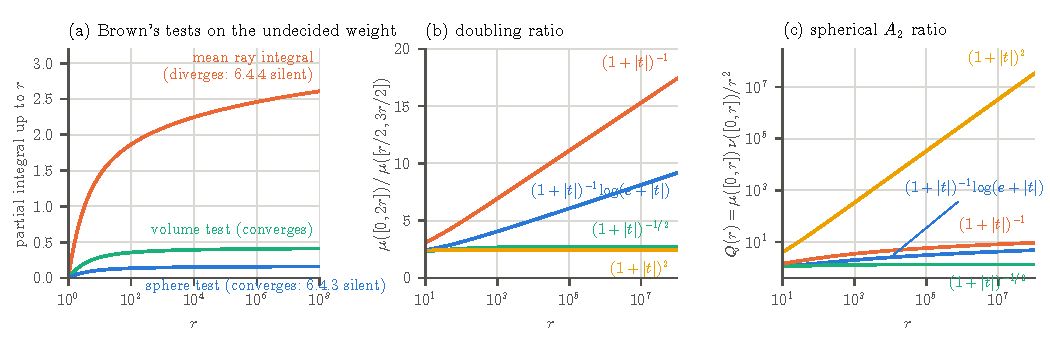
\includegraphics[width=\textwidth]{fig2_undecided.pdf}
\caption{(a) Brown's radial tests on the weight of Example~\ref{ex:log}:
the sphere-average integral converges (Theorem 6.4.3 silent), the
direction-averaged ray integral diverges like $\log\log r$ (Theorem
6.4.4 silent), and the volume integral converges. (b) The doubling ratio
$\mu([0,2r])/\mu([r/2,3r/2])$ of four weights: bounded for
$(1+\abs t)^{-1/2}$ and $(1+\abs t)^2$, growing like $\log r$ for the two
borderline weights, which are therefore not doubling. (c) The
spherical $A_2$ ratio $Q(r)$: bounded only for $(1+\abs t)^{-1/2}$, the
one weight that is both doubling and Poincar\'e (Lemma~\ref{lem:k9});
$(1+\abs t)^2$ is doubling but fails the Poincar\'e inequality. All
curves are recomputed from the scripts of record.}
\label{fig:undecided}
\end{figure*}

\begin{lemma}[spherical $A_2$ makes the radial tests exhaustive]
\label{lem:k8}
Suppose $\sup_{r\ge1}Q(r)=C<\infty$. If
$\int_1^\infty\dd r/(r^{m-1}\fbar(r))=\infty$, then $W_F$ is parabolic
and $\delta_F$ is admissible whenever $\gamma_F$ is bounded. If the
integral is finite, $\delta_F$ is inadmissible.
\end{lemma}

\begin{proof}
The first case is Theorem~\ref{thm:brown}(d). In the second, let
$R(\varphi)=\int_1^\infty\dd r/(r^{m-1}f^*(r\varphi))$. By Fubini its
mean over the unit sphere is
$\int_1^\infty A(r)\dd r/r^{m-1}\le C\int_1^\infty\dd r/(r^{m-1}\fbar(r))<\infty$,
so by Chebyshev the set $\Omega=\{\varphi:R(\varphi)\le2\,\mathrm{mean}\,R\}$
has at least half the surface measure and $R$ is bounded on it. This
is the hypothesis of Theorem~\ref{thm:brown}(e).
\end{proof}

Brown's own remark after his Theorem~6.4.4 already contains the Fubini
form of (e) and the Jensen inequality $A(r)\ge1/\fbar(r)$; the lemma
only observes that a bounded ratio closes the gap. Consequently every
weight on which both tests are silent has $Q(r)\to\infty$ along some
sequence: unbounded contrast between the arithmetic and harmonic sphere
means of $f^*$.

\begin{lemma}[doubling and Poincar\'e force $A_2$ on centred intervals]
\label{lem:k9}
Let $w>0$ be continuous on $\R$, $\mu=w\dd t$, $\nu=w^{-1}\dd t$.
Suppose $\mu$ is doubling, $\mu(2I)\le D\,\mu(I)$ for every interval
$I$, and satisfies the scale-invariant Poincar\'e inequality
$\int_I\abs{u-u_I}^2\dd\mu\le C\abs{I}^2\int_I\abs{u'}^2\dd\mu$ for all
$I$ and smooth $u$. Then $\mu([-r,r])\,\nu([-r,r])\le 32\,CD^3\,r^2$
for every $r>0$.
\end{lemma}

\begin{proof}
Take $I=[-2r,2r]$ and the test function $u=0$ on $[-2r,-r]$, $u=1$ on
$[r,2r]$, and $u(t)=\nu([-r,t])/\nu([-r,r])$ in between, which
minimizes the energy across the middle segment:
$\int_I\abs{u'}^2\dd\mu=1/\nu([-r,r])$. A function equal to $0$ on a
set of measure $a$ and to $1$ on a set of measure $b$ has weighted
variance at least $ab/(a+b)\ge\tfrac12\min(a,b)$. Since $[-r,r]$ is
contained in the eightfold dilates of $[r,2r]$ and of $[-2r,-r]$,
doubling gives $\mu([r,2r])\ge\mu([-r,r])/D^3$, and likewise for
$\mu([-2r,-r])$. The Poincar\'e inequality now reads
$\mu([-r,r])/(2D^3)\le C(4r)^2/\nu([-r,r])$.
\end{proof}

Both hypotheses are needed (Table~\ref{tab:weights},
Fig.~\ref{fig:undecided}b,c): $(1+\abs t)^2$ is doubling but fails the
Poincar\'e inequality, because the valley at $0$ is a bottleneck
between two heavy sides, and its ratio grows like $r/3$;
$(1+\abs t)^{-2}$ satisfies the Poincar\'e inequality but is not
doubling, and its ratio also grows like $r/3$.

\begin{corollary}[product weights]\label{cor:product}
Let $m\ge3$ and let $f^*(x)=w(x_1)$, or its Gaussian smoothing, with
$w$ as in Lemma~\ref{lem:k9}. Then $Q(r)$ is bounded, so
Lemma~\ref{lem:k8} applies; in fact $\delta_F$ is inadmissible by
Theorem~\ref{thm:brown}(e), and the volume-growth criterion of
Remark~\ref{rem:volume} decides nothing that Brown's two tests do not.
\end{corollary}

\begin{proof}
The sphere means of $w(x_1)$ are weighted means of $w$ over $[-r,r]$
with a bounded kernel that is bounded below on $[-r/\sqrt2,r/\sqrt2]$,
so by doubling $\fbar(r)\asymp\mu([-r,r])/r$ and
$A(r)\lesssim\nu([-r,r])/r$; Lemma~\ref{lem:k9} bounds $Q$. Doubling
also gives $\mu([-r,r])\ge c\,r^{\varepsilon}$ for some
$\varepsilon>0$ (reverse doubling), so the sphere integral
$\int^\infty\dd r/(r^{m-1}\fbar)$ is dominated by
$\int^\infty r^{2-m-\varepsilon}\dd r<\infty$ for $m\ge3$, and the
second case of Lemma~\ref{lem:k8} applies.
Gaussian smoothing changes $w$ by a bounded factor when $\log w$ has a
bounded derivative, and changes nothing above.
\end{proof}

\begin{remark}[the volume criterion, conditional]\label{rem:volume}
Under doubling and a scale-invariant Poincar\'e inequality on balls,
the Dirichlet form of $W_F$ satisfies the parabolic Harnack inequality
and two-sided Gaussian heat-kernel bounds
\cite{grigoryan1991,saloffcoste1992,sturm1996} (Muckenhoupt $A_2$
weights are an example \cite{fks1982}), and then transience is
equivalent to $\int^\infty r\dd r/\mu(B(0,r))<\infty$
\cite[Thm.\ 11.1 and its proof]{grigoryan1999}. Combined with
Theorem~\ref{thm:brown}(b) this would be an admissibility criterion
for $W_F$. Corollary~\ref{cor:product} shows it is empty of new content
for product weights. Whether a non-product doubling--Poincar\'e weight
exists on which both of Brown's tests are silent is open: the
one-dimensional mechanism is excluded by Lemma~\ref{lem:k9}, but in
$\R^m$ an escape route that is cheap without being radial is not
excluded by our argument, and we found no example. An earlier internal
record of this gate asserted the bound of Lemma~\ref{lem:k9} for the
whole class without proof; that step is withdrawn and replaced by the
lemma.
\end{remark}

\begin{example}[an undecided weight, decided]\label{ex:log}
Let $F(\dd\theta)=(1+\abs{\theta_1})^{-1}\log(e+\abs{\theta_1})\,
\dd\theta_1\dd\theta_2\dd\theta_3$ on $\R^3$, so that $f^*$ depends on
$x_1$ only, $\gamma_F$ is bounded, and
$f^*\asymp(1+\abs{x_1})^{-1}\log(e+\abs{x_1})$.
Theorem~\ref{thm:brown}(d) is silent: $\fbar(r)\asymp\log^2r/r$ and
the sphere integral converges. Theorem~\ref{thm:brown}(e) is silent:
along a direction with $\cos\varphi\ne0$ the ray integral is
$\abs{\cos\varphi}\int^\infty\dd r/(r\log r)=\infty$, and the
equatorial directions have measure zero; (f) does not apply since
$\gamma_F\asymp1/\abs{x_1}$ is not $O(1/\abs x)$. The weight is not
doubling either, its doubling ratio grows like $\log r$
(Fig.~\ref{fig:undecided}b), so Remark~\ref{rem:volume} does not apply,
although its integral happens to converge. The product structure
decides: $\{Z_t\}$ is the product of the one-dimensional diffusion $W$
with generator $w^{-1}(wu')'$ and a Brownian motion on $\R^2$, and
$\{Z_t\}$ is transient iff $\int^\infty p^W_t(0,0)\,(4\pi t)^{-1}\dd t<\infty$.
A Crank--Nicolson computation of $p^W_t(0,0)$ (density with respect to
$w\dd t$; the control $w\equiv1$ reproduces $(4\pi t)^{-1/2}$ to five
digits) gives $\log^2\!t\cdot p^W_t(0,0)=2.58,\,2.95,\,3.18,\,3.33,\,3.44$
at $t=10^3,\dots,10^7$, i.e.\ $p^W_t(0,0)\asymp1/\log^2t$, as the
null-recurrent heuristic $p^W_t(0,0)\approx1/\mu([-\sqrt t,\sqrt t])$
predicts. Hence the integral converges, $\{Z_t\}$ is transient and
$\delta_F$ is inadmissible by Theorem~\ref{thm:brown}(b). A rigorous
citation for the one-dimensional asymptotic is owed before the example
is used elsewhere. The method is the one with which Johnstone and
Lalley \cite{johnstonelalley1984} answered Brown's question (his
\S6.5) whether any non-proper-Bayes estimator is immune to the Stein
effect under products; the example is an instance of their phenomenon:
a recurrent one-dimensional generalized Bayes piece whose product with
the admissible two-dimensional MLE is inadmissible.
\end{example}

\section{Four geometries, no horizon, no dynamics}\label{sec:geoms}

The phrase ``interior geometry'' in the blueprint denoted four
different objects, and every one of its physical claims came from
conflating them. (1)~The Fisher--Rao metric of the model: flat for the
normal location family, hyperbolic for a location--scale family
(Komaki's Example~2); for $N(\mu,\sigma^2)$, $g=\mathrm{diag}(1/\sigma^2,
2/\sigma^2)$ with curvature $-1/2$ (check C22). This is the horn of
Fig.~\ref{fig:geom}a: the throat is $\sigma\to\infty$, the flare
$\sigma\to0$, and the axial coordinate $-\ln\sigma\approx\tfrac12\ln N$
is an observation count, an \emph{external} clock. Its curvature is the
model's; the curvature in \S\S\ref{sec:komaki}--\ref{sec:brown} is the
prior's. (2)~The weighted manifold $(M,g,e^{-\Phi}\dd V)$, where
Propositions~\ref{prop:k1}--\ref{prop:k2} and Theorem~\ref{thm:brown}
live. (3)~Komaki's conformal frame, Fig.~\ref{fig:geom}b, in which the
Stein prior becomes a flat cylinder with the origin at infinite
distance. (4)~The pullback $J^\top\Sigma^{-1}J$ of the estimator map
(check C11), a legitimate Riemannian object on the data space whose
angular part degenerates at $\norm x=\sigma\sqrt{d-2}$ for the
James--Stein map, where its tangential Jacobian eigenvalue vanishes and
the radial one equals~2 (check C12; Fig.~\ref{fig:geom}c). This is the
only ``horizon'' in sight, and it is a statement about an estimator,
not about causal structure; no Schwarzschild form arises (check C3).

There is no dynamics. In Perelman's $\mathcal F$ the measure is a gauge
and the metric flows; in statistics the Fisher metric is fixed by the
model and all content sits in the measure, which Bayesian updating
moves at fixed $g$ through $f_N\propto f\,L_N$, a log-likelihood
increment and not a Ricci-type flow. The Bakry--\'Emery flow of
Table~\ref{tab:dict} therefore has no statistical process generating
it as the framework stands, and any future dynamical claim must supply
a mechanism that changes $g$ and must declare its clock.

\section{Assessment and record}\label{sec:record}

What this note can claim: the dictionary of Table~\ref{tab:dict};
Proposition~\ref{prop:k1} with its sign; Proposition~\ref{prop:k2} as
the reason the dictionary stops at the gradient term;
Theorem~\ref{thm:brown} as the geometric reading of a formulation that
statistics already owns in Dirichlet-form language;
Remark~\ref{rem:k7} as a historical observation; Lemmas
\ref{lem:k8}--\ref{lem:k9} as corollaries of Brown's theorems. What it
cannot claim: any gravitational or dynamical statement; the words
``horizon'', ``Einstein frame'' or ``spacetime'' except as names of
functional forms; any novelty wording before a citation-index sweep.
The owner's assessment of record is that nothing here rises to a
contribution; the research question that the dictionary left behind,
a new admissibility criterion from weighted potential theory, closed
on its first serious test (\S\ref{sec:reach}) with one small open
residue (Remark~\ref{rem:volume}). The stream is closed and this note
is its record.

\paragraph{Verification record.}
Equation lint: 22 symbolic and Monte Carlo checks
(\path{checks/lint_admissible_spacetime.py}; 6 FAIL on the
blueprint's claims, 12 PASS, 4 INFO). Bibliography: 24 references of
the blueprint checked field by field against publisher, Crossref or
arXiv records (22 verified, 1 with corrections, 1 unverified).
Numerics: \path{checks/g0_feasibility.py} (sphere, ray and volume
integrals; Crank--Nicolson heat kernel) and
\path{checks/g0_doubling_poincare.py} (doubling ratios,
Muckenhoupt--Hardy bounds, spherical ratios); every number in
Table~\ref{tab:weights} and Fig.~\ref{fig:undecided} is produced by
these scripts. Brown~\cite{brown1971} was read from a scan of the
journal pages; its theorems are cited by their numbers there.

\bibliographystyle{unsrt}
\bibliography{references}

\end{document}
